% Figures/research_overview.tex
\begin{figure}[ht]
    \centering
    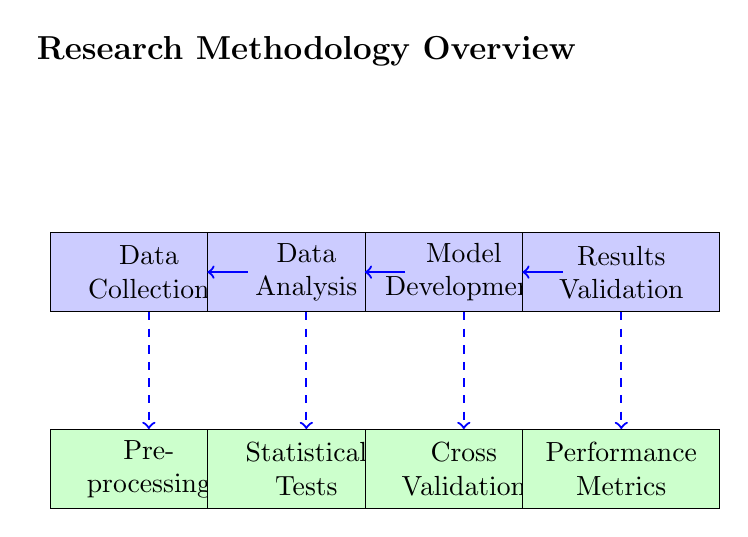
\begin{tikzpicture}[
            node distance=2cm,
            box/.style={rectangle, draw, fill=blue!20, minimum width=2.5cm, minimum height=1cm, align=center},
            arrow/.style={->, thick, blue}
        ]

        % Main process boxes
        \node[box] (data) {Data\\Collection};
        \node[box, right of=data] (analysis) {Data\\Analysis};
        \node[box, right of=analysis] (model) {Model\\Development};
        \node[box, right of=model] (results) {Results\\Validation};

        % Arrows between boxes
        \draw[arrow] (data) -- (analysis);
        \draw[arrow] (analysis) -- (model);
        \draw[arrow] (model) -- (results);

        % Sub-processes
        \node[box, fill=green!20, below of=data, yshift=-0.5cm] (preprocessing) {Pre-\\processing};
        \node[box, fill=green!20, below of=analysis, yshift=-0.5cm] (statistics) {Statistical\\Tests};
        \node[box, fill=green!20, below of=model, yshift=-0.5cm] (validation) {Cross\\Validation};
        \node[box, fill=green!20, below of=results, yshift=-0.5cm] (evaluation) {Performance\\Metrics};

        % Connecting sub-processes
        \draw[arrow, dashed] (data) -- (preprocessing);
        \draw[arrow, dashed] (analysis) -- (statistics);
        \draw[arrow, dashed] (model) -- (validation);
        \draw[arrow, dashed] (results) -- (evaluation);

        % Title
        \node[above of=analysis, yshift=0.8cm, font=\large\bfseries] {Research Methodology Overview};

    \end{tikzpicture}
    \caption{Lorem ipsum dolor sit amet research methodology flowchart showing the main phases of the study process.}
    \label{fig:research_overview}
\end{figure}